\documentclass{article}

\usepackage[final,dblblindworkshop]{neurips_2026}
\workshoptitle{AI-Native Academia: Authorship, Peer Review, and Conference Governance under AI}

\usepackage[utf8]{inputenc}
\usepackage[T1]{fontenc}
\usepackage{hyperref}
\usepackage{url}
\usepackage{booktabs}
\usepackage{amsfonts}
\usepackage{amsmath}
\usepackage{nicefrac}
\usepackage{microtype}
\usepackage{xcolor}
\usepackage{graphicx}
\usepackage{array}
\usepackage{tabularx}
\usepackage{ragged2e}
\usepackage{longtable}
\usepackage{placeins}

\newcommand{\ImplementationTestsCaption}{Decisions on 52 of the 60 implementation cases. The eight conformant original cases are reported in the supplementary results table. Blue marks the expected decision, orange a missed fault or false alarm, and gray unavailable coverage.}

\newcommand{\AgentPRMTargetsCaption}{AgentPRM targets before and after correcting the discount exponent. The left panel shows signed targets for an eight-state successful trajectory at $\gamma=0.95$. The right panel shows the largest change in exported targets across trajectory lengths. Exported targets use $0.5(Q+1)$, giving half the change in signed targets.}

\newcommand{\ToolACEMaskCaption}{ToolACE mask alignment after left cropping. Ten prompt tokens and four response/EOS tokens are cropped to eight inputs, removing six prompt tokens. The mask at position $i$ weights the prediction of retained token $i+1$. The original mask suppresses all four response/EOS predictions; the corrected mask retains them. Padding and the final position with no next-token prediction are excluded.}

\newcommand{\AgentAbstainWeightingCaption}{Released subtype counts and the maximum absolute difference between equal-subtype and pair-weighted scenario averages. Constructed outcomes attain the overall bound of 2.412476 percentage points through the unchanged evaluator and ranking computation.}

\newcommand{\ToolACELengthCaption}{Sequence lengths for the 9,394 converted examples with nonempty responses. The 570 EOS-only examples are omitted from the histogram. All 9,964 converted examples were checked against the 8,192-token limit; none exceeded it, and the maximum length was 3,945 tokens.}

\newcommand{\MissingPairsCaption}{Maximum weighting difference after hypothetical removal of zero, one, three, or eight complete pairs from one subtype in each scenario. The removed subtype is chosen separately for each scenario to maximize the difference. Removing pairs simultaneously across the eight scenarios gives overall bounds of approximately 2.41, 4.07, 7.71, and 19.43 percentage points.}


\title{Executable Scientific Contracts for Verifiable LLM and Agent Research}

\author{Amir Reza Peimani\\University of Toronto\\\texttt{amir.peimani@utoronto.ca}}


\usepackage{listings}
\usepackage{needspace}
\raggedbottom
\hypersetup{hidelinks,pdftitle={Executable Scientific Contracts for Verifiable LLM and Agent Research},pdfauthor={Amir Reza Peimani}}
\lstset{basicstyle=\ttfamily\footnotesize,breaklines=true,columns=fullflexible,keepspaces=true,showstringspaces=false,frame=none,aboveskip=5pt,belowskip=5pt}

\begin{document}
\maketitle

\begin{abstract}
Research audits often uncover code discrepancies whose effects on reported results remain unclear. We study executable scientific contracts: checks that connect a paper claim, its implementation, a controlled input, and evidence from released artifacts. We examine 25 checks across five agent and language model repositories. In tests of upstream implementations, the contracts detected all 17 faulty variants, accepted all three repairs, and raised no flags on 12 harmless rewrites. In AgentPRM, correcting a temporal error changes state targets and preference construction while preserving the mean over complete trajectory visits. ToolACE's crop defect is inactive across 9,964 examples produced by the official conversion. In AgentAbstain, the released task composition permits a maximum difference of 2.4125 percentage points between two weighting conventions. These cases show how executable checks distinguish implementation errors, inactive defects, and unspecified evaluation choices, giving reviewers reproducible evidence for assessing an audit finding.
\end{abstract}

\section{Introduction}
Language models increasingly assist scientific writing, code inspection, and peer review. An audit finding still needs a precise connection to the paper's computation and data. We study checks that make this connection executable and show which conclusions the available artifacts support.

Reproducibility taxonomies distinguish repeatability and reconstruction \citep{tatman2018taxonomy}. Algorithmic unit tests and mutation testing examine implementation behavior and the ability of tests to detect faults \citep{raff2023algorithmic,just2014major,panichella2021mutation,tufano2019mutate}. Guidelines for agent benchmarks also address evaluation quality \citep{zhu2025agentbenchmarks}.

RepoAudit uses LLM agents to audit repositories \citep{guo2025repoaudit}. SciCoQA evaluates scientific paper--code alignment using verified mismatch reports \citep{baumgartner2026scicoqa}. AuditOwl extracts paper claims, traces them to code, and verifies candidate discrepancies with executable checks \citep{auditowl2026}. SANA generates contracts for scientific data-analysis workflows \citep{sana2026}.

Rules to Tools supplies executable scientific checks for coding agents \citep{ning2026rules}. ReproAgent maintains implementation requirements during paper-to-code reproduction \citep{hu2026reproagent}. Semantic Mutation Score evaluates test adequacy using mutations based on scientific semantics \citep{li2026semanticmutation}.

Following design by contract \citep{meyer1992contract}, we record an audit finding as an executable check of the stated behavior. Each contract connects the claim, implementation, test input, activation in released data, and evidence about the reported result. We examine 25 checks across five repositories and evaluate how the checks respond to faults, repairs, and harmless changes.

\section{Executable scientific contracts}

\paragraph{Contract contents.}
A contract records the statement or equation being checked, the implementing code, an input that distinguishes expected from implemented behavior, whether the relevant condition occurs in released data, and the evidence connecting the finding to a reported result. We organize these records as
\[
\text{claim} \rightarrow \text{implementation} \rightarrow
\text{controlled check} \rightarrow \text{activation} \rightarrow
\text{result evidence}.
\]

\paragraph{Outcome labels.}
Conformant means that the implementation matches the stated expectation on the tested input. Discrepant means that the check exposes a mismatch. Inactive means that a demonstrated defect is not triggered in the inspected released data. Convention sensitivity means that the source leaves a choice unspecified and reasonable alternatives produce different values. We record implementation behavior, eligible examples, activation, and the connection to a reported result separately.

\paragraph{Case selection.}
We retained five checks for each of AgentPRM \citep{choudhury2025agentprm}, ContractBench \citep{contractbench2026}, ToolACE \citep{liu2024toolace}, $\tau$-bench \citep{yao2025taubench}, and AgentAbstain \citep{liu2026agentabstain}. The first four cases revisit earlier audit findings. Their 20 checks were constructed with those findings already known. The records do not specify a stopping rule for the retrospective selection. The five AgentAbstain checks were specified before execution. The inventory includes substantive checks, consistency checks, and summaries, covering equations, schemas, logging, aggregation, and data support. Repository revisions and the complete inventory appear in the supplement.

\paragraph{Selecting a new contract.}
We recommend starting with a claim central to a reported result. Locate the implementing computation and construct an input that distinguishes the stated behavior from a plausible error. Then check whether that input condition occurs in the released data.

\paragraph{Implementation tests.}
The checks execute pinned upstream functions or unchanged function extractions whose hashes are recorded. We compare field/type validation, the original adapters, and contracts that test function behavior. The original adapters combine source inspection with locally reconstructed calculations. The faults preserve the required fields and types. The original-adapter comparison covers AgentPRM and ToolACE; relevant native test coverage was unavailable for the selected behaviors.

The experiment contains 60 cases: 17 faulty variants, comprising three original faults and 14 injected variants; three repairs; 12 harmless rewrites; eight conformant original cases; and 20 cases with missing evidence or ineligible inputs. A shared check returns `not evaluated' when required evidence is missing or no eligible examples are available, before the compared methods run. We reran the same 60 cases after correcting the eligibility checks and prediction-mask accounting.

After freezing the corrected checks, we constructed nine additional cases covering terminal-reward remapping, response-token order, and replacement of the outer scenario mean with a median. Each family contains a fault, a reference implementation, and a harmless rewrite. The checks and their imports remained unchanged. These nine cases are reported separately.

The earlier mutation experiment exercised four fixture validators. Its 30 mutations and the eight externally motivated operators are documented in the supplement.

\par\noindent\begin{minipage}{\linewidth}
\paragraph{Complete executable example.}
The AgentAbstain conjunction check uses the four Boolean act/abstain pairs, for which paired accuracy is 0.25. The listing constructs the evaluator input and calls \texttt{compute\_summary\_metrics} from revision f5812497. Code, study artifacts, environment specifications, and run commands are available at \url{https://github.com/AmirRezaPeimani/executable-scientific-contracts}.
\lstinputlisting{../scripts/agentabstain_contract_example.py}
The check prints `paired\_accuracy: 0.25 PASS' and the SHA-256 hash of the imported source file.
\end{minipage}\par

\section{Results}

\paragraph{Implementation tests.}
Figure~\ref{fig:implementation-tests} compares decisions on faulty implementations, repairs, and harmless rewrites. Acceptance of repaired code and harmless rewrites was the clearest improvement over the original adapters. The field/type checks accepted the faulty outputs because their fields and types were preserved. The 20 cases with missing evidence or ineligible inputs exercised the shared check that returns `not evaluated'.

The frozen checks also distinguished the faults, reference implementations, and harmless rewrites in the nine additional cases. Table~\ref{tab:additional-families} reports these results separately.


\begin{figure}[!htbp]
\centering
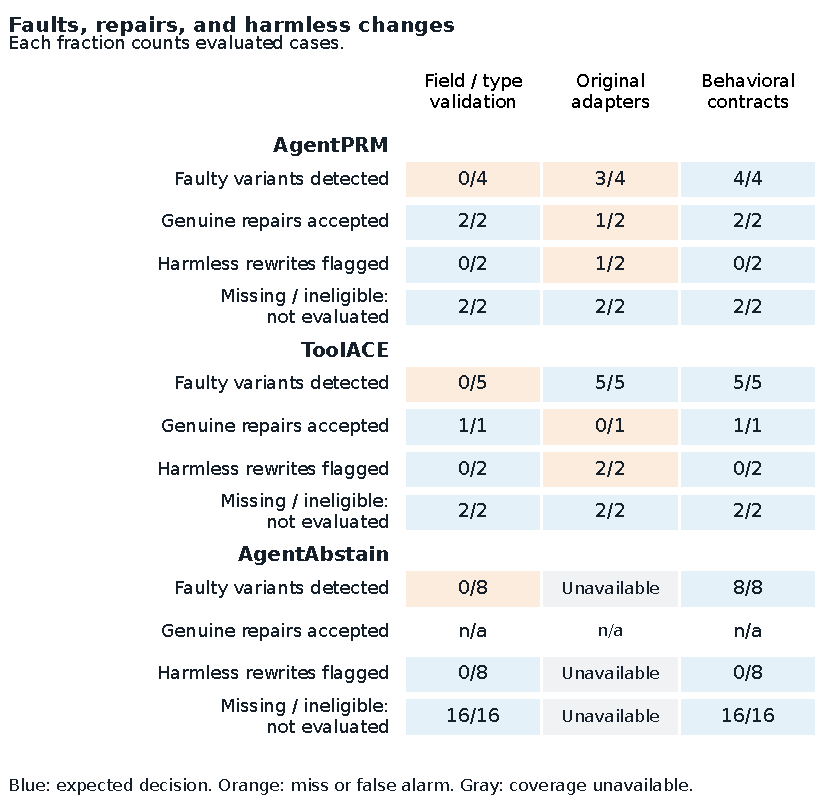
\includegraphics[width=\linewidth]{../figures/behavior_matrix.pdf}
\caption{\ImplementationTestsCaption}
\label{fig:implementation-tests}
\end{figure}
\FloatBarrier


\begin{table}[!htbp]
\centering
\small
\setlength{\tabcolsep}{3pt}
\caption{Nine cases constructed after the checks were frozen. Each mutation family contains a fault, a reference implementation, and a harmless rewrite.}
\label{tab:additional-families}
\begin{tabularx}{\linewidth}{@{}>{\RaggedRight\arraybackslash}p{0.19\linewidth}*{4}{>{\RaggedRight\arraybackslash}X}@{}}
\toprule
Method & Faults detected & References accepted & Benign flags & Uncovered faults \\
\midrule
Field/type & 0/3 & 3/3 & 0/3 & 0 \\
Native tests & Unavailable & Unavailable & Unavailable & 3 \\
Original adapters & 2/2 covered & 0/2 covered & 2/2 covered & 1 \\
Behavioral contracts & 3/3 & 3/3 & 0/3 & 0 \\
\bottomrule
\end{tabularx}
\par\smallskip\noindent
All nine cases completed and were included. The checks and their imports matched the recorded hashes.
\end{table}

\FloatBarrier

\Needspace{3.5in}
\paragraph{AgentPRM: temporal targets.}
AgentPRM's target equation discounts a terminal reward by remaining trajectory length, while both target callers pass the forward time index. For a successful four-action trajectory at the released $\gamma=0.95$, correcting the callers changes the signed targets from $(1,0.95,0.9025,0.857375)$ to $(0.857375,0.9025,0.95,1)$. The mean remains 0.92746875, but the target assigned to each state changes.

Reversal preserves the multiset over complete trajectory visits. Averaging deduplicated state-action targets can give different means before and after repair. The absolute-target exporter applies $0.5(Q+1)$; preference construction uses the signed values. For two successful continuations from a shared state, with lengths four and eight, the signed margin changes from zero to $0.95^3-0.95^7$, exceeding the released preference threshold $\delta=0.03$. A preference is added for each of the 28 chosen length pairs. Figure~\ref{fig:agentprm-targets} shows how target assignment changes with trajectory position and length.

The rollout also copies observations into the action field of the query history. A test agent records six incorrect history entries before repair and none afterward. The separately saved trajectory contains the executed actions in both versions. Historical training traces were unavailable.


\begin{figure}[!htbp]
\centering
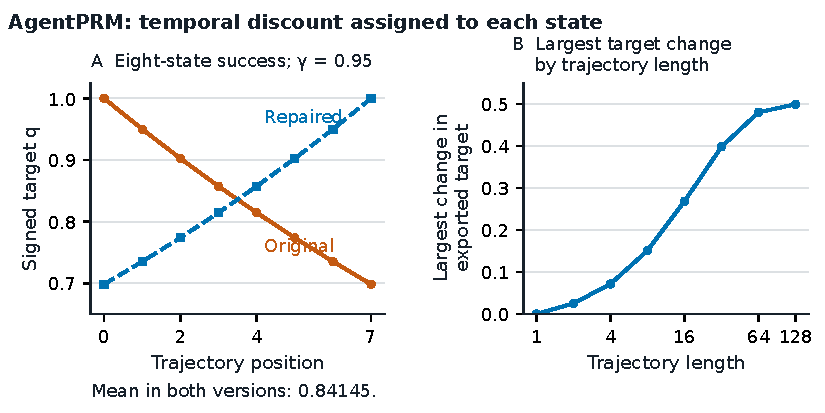
\includegraphics[width=\linewidth]{../figures/agentprm_trajectory.pdf}
\caption{\AgentPRMTargetsCaption}
\label{fig:agentprm-targets}
\end{figure}
\FloatBarrier


\paragraph{ToolACE: cropping and released data.}
ToolACE's loader constructs the response mask using coordinates from before left cropping. In the controlled example, cropping a sequence of ten prompt tokens and four response/EOS tokens to eight inputs removes all supervision under the original mask. Correcting the coordinates restores four supervised predictions. Figure~\ref{fig:toolace-mask} shows the alignment between retained inputs, next-token labels, and mask positions.

The official conversion produces 9,964 examples. Running the loader with the recorded tokenizer finds no sequence above the 8,192-token limit; the maximum length is 3,945. The crop defect is therefore inactive on these converted examples. The supplement reports the conversion counts, excluded candidates, and differences from the earlier custom converter.


\begin{figure}[!htbp]
\centering
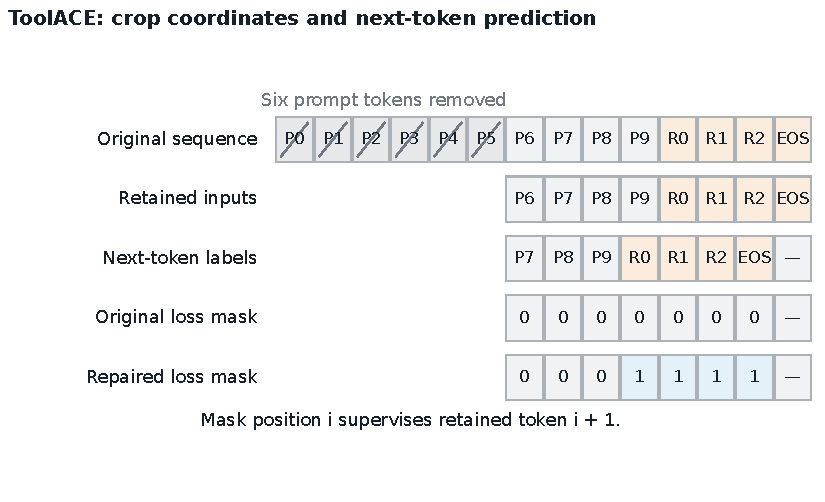
\includegraphics[width=\linewidth]{../figures/toolace_prediction_mask.pdf}
\caption{\ToolACEMaskCaption}
\label{fig:toolace-mask}
\end{figure}
\FloatBarrier


\paragraph{ContractBench: released evaluation records.}
ContractBench reports 56.6\% for Qwen3.5-9B on 99 tasks. The released artifact contains 0/99 success labels under the repository mapping. Three traces report 8,192 output tokens but contain no terminal assistant response. The model name and evaluation size match the report; the original checkpoint, task set, and evaluation configuration remain unverified. The successful-trace check has zero eligible examples and is marked `not evaluated'.

\paragraph{AgentAbstain: metric conventions.}
AgentAbstain's released task file contains 526 rows forming 263 complete act/abstain pairs across eight scenarios. Pair integrity, paired-accuracy conjunction, and commit scoring match the source. Two choices remain unspecified: the treatment of an empty conditioned denominator and the weighting of subtypes within a scenario.

For subtype fraction $w$ and success rates $p_1,p_2$, the difference between equal-subtype and pair-weighted averages is
\[
\Delta=(1/2-w)(p_1-p_2).
\]
The released subtype counts permit a maximum absolute difference of 2.412476 percentage points in the overall eight-scenario macro average. Individual scenario bounds range from zero to 5.882353 points. Constructed endpoint outcomes attain the overall bound through the unchanged ranking computation. Figure~\ref{fig:agentabstain-weighting} shows the counts and scenario bounds. Released model outputs were unavailable.


\begin{figure}[!htbp]
\centering
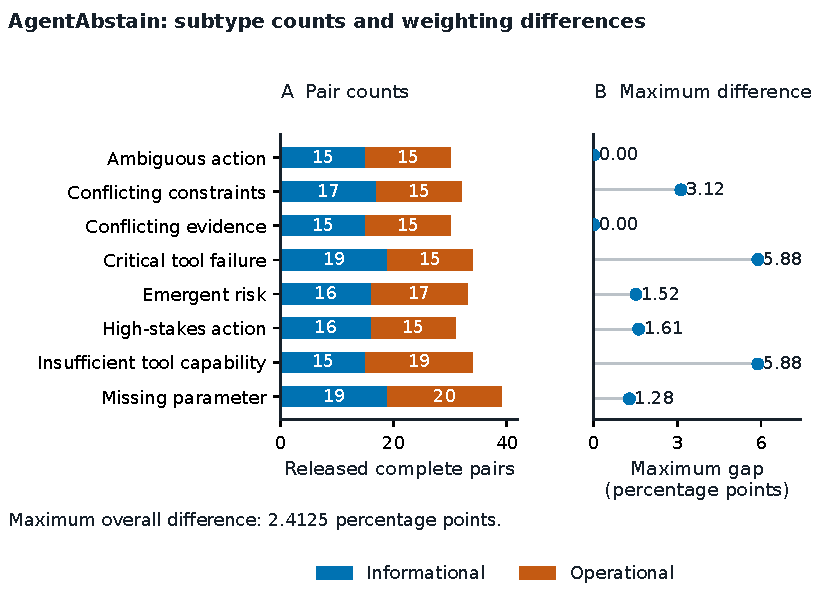
\includegraphics[width=\linewidth]{../figures/agentabstain_composition_bounds.pdf}
\caption{\AgentAbstainWeightingCaption}
\label{fig:agentabstain-weighting}
\end{figure}
\FloatBarrier


\paragraph{Execution time.}
The original suites were quick to rerun once implemented. Timings include process startup and reading saved summaries; data acquisition, conversion, and the full ToolACE scan were outside the measurement. The supplement reports all timing measurements.

\section{Implications for AI-native academia}
We propose attaching executable contracts to the main quantitative claims in a submission. Authors would provide the inputs, expected outputs, source versions, and run commands. Reviewers and auditing tools could rerun these checks and add cases that probe the claim.

\paragraph{Limitations.}
The study covers five repositories and manually selected faults. The checks and outcome labels were assigned by one author. Authoring time and agreement between independent authors were not measured. The proposed review workflow has not been evaluated in use.

\section{Conclusion}
Checks that execute upstream code can detect faults while accepting repairs and harmless rewrites. Together with checks of released data, they provide a practical record of what an audit found and how to reproduce it.
\label{end-of-main-text}
\clearpage\bibliographystyle{plainnat}\bibliography{references}
\end{document}
